\section{Creation of a block in GNU Radio}

The easiest way to create a new GNU Radio block in our case is to copy an existing one. For the sake of simplicity, it is preferable to use the same name as the block label and as the name of the block files, here \textit{\textbf{test\_block}}. A GNU radio block is identified and described by a YAML file. In our case they are located in the \texttt{gr-fsk/grc} directory. It starts by providing the block ID which you should modify to \textit{fsk\_test\_block}. The different parameters, inputs and outputs of your block must be given as it is done in various blocks of the gr-fsk library. Finally the make command links the YAML description to the software implementation, here mainly in Python. The implementation will be part of the \texttt{fsk} package and the make command in YAML file will therefore be \textit{fsk.test\_block}. It is followed by the different parameters you registered to link them with the Python implementation. An example is shown in Fig. \ref{fig:Basic_yml}.

\begin{figure}[h]
    \centering
    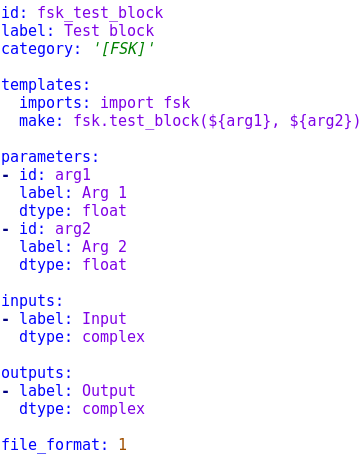
\includegraphics[scale=0.8, left]{figures/Basic_yml.png}
    \caption{Basic YAML file describing a block}
    \label{fig:Basic_yml}
\end{figure}

You can also start the Python implementation by copying the one of another block. The name of the class must match the \textbf{test\_block} used in the YAML file. The constructor of the class (\textit{\_\_init\_\_} function) takes the block parameters as arguments. Also, it uses the parent class \textit{gr.basic\_block}. You must refer your input and output types in this call. The corresponding example is shown in Fig. \ref{fig:Basic_python}.

\begin{figure}[h]
    \centering
    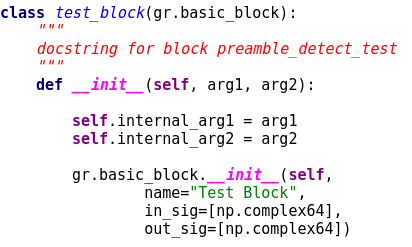
\includegraphics[scale=0.75, left]{figures/Basic_python.png}
    \caption{Basic Python constructor of a GNU Radio block}
    \label{fig:Basic_python}
\end{figure}

In order for the block to be properly compiled and linked, you must also make modifications to the following files:

\begin{itemize}
    \item \texttt{gr-fsk/python/\_\_init\_\_.py}  : add \textit{from .test\_block import test\_block}
    \item \texttt{gr-fsk/python/CMakeLists.txt}  : add \textit{test\_block.py} next to the other blocks
    \item \texttt{gr-fsk/grc/CMakeLists.txt}  : add \textit{fsk\_test\_block.block.yml} next to the other blocks
\end{itemize}

When all the steps have been done, you need to recompile the library by going in the \texttt{gr-fsk/build} directory and run:
\begin{lstlisting}[language=bash]
    $ cmake ..
    $ sudo make install
\end{lstlisting}



\section{Dynamic update of a GNU Radio variable}

To do this, the GNU Radio block will perform a callback to a high level function that will update a variable of the Graph. We have to change both the YAML file of the block and its Python code. For the Python code, the block \textit{\_\_init\_\_} function takes a new argument \textit{callback}, as shown below.

 \begin{figure}[H]
    \centering
    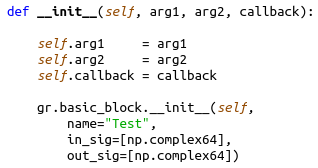
\includegraphics[scale=0.65, left]{figures/Callback_python.png}
    \caption{Constructor of the block Python class}
    \label{fig:callback_python}
\end{figure}

You can then use this callback function inside the block implementation to update the variable, by simply using \texttt{self.callback(value)}

Next, in the YAML file of the block, we need to add a parameter to the block which is the variable to modify, here \textit{var\_to\_update}. Be careful that it must be referenced as a string. We also need to add a specific part to the make command, to link the variable name and the high level function that is used to perform the update. Here is the part of command to add:

\begin{lstlisting}[language=bash]
    { 'self.set_' + context.get('var_to_update')() }
\end{lstlisting}

The name used in this part of command must match the new parameter \textit{var\_to\_update}. In the case of the test block provided in this tutorial, the resulting start of YAML file is shown in Fig. \ref{fig:Callback_yml}

 \begin{figure}[H]
    \centering
    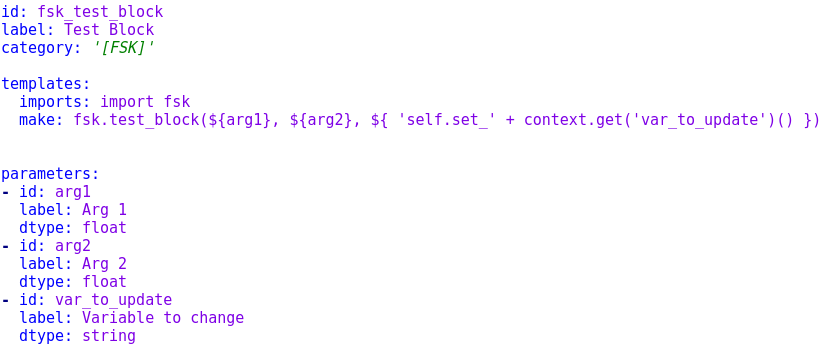
\includegraphics[scale=0.45, left]{figures/Callback_yml.png}
    \caption{Example of YAML file of a block with a variable update (inputs ant outputs are missing) }
    \label{fig:Callback_yml}
\end{figure}

Do not forget to recompile the gr-fsk library after making any modifications to a block, otherwise your changes won't propagate. You can then reopen GNU radio and your Graph. The last step is to create a new variable in the Graph and to add it in your modified block parameters, as shown in Fig. \ref{fig:Callback_graph}

 \begin{figure}[H]
    \centering
    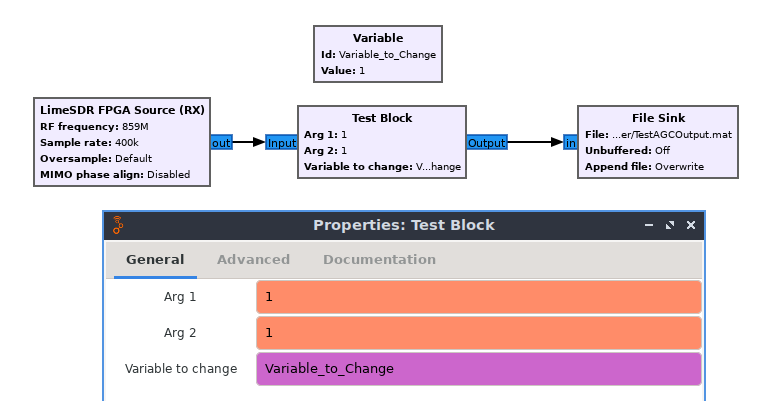
\includegraphics[scale=0.55]{figures/Callback_graph.png}
    \caption{Modifications to make to the GNU Radio Graph}
    \label{fig:Callback_graph}
\end{figure}

\section{Get the updated value of a GNU Radio variable}

When instantiating a GNU Radio and providing it with parameters, there are only read once when creating the block. We need to do small modifications to ensure the block internal value is updated each time we modify the variable value as explained in the previous section. The LimeSDR block in GNU Radio already handles this but the following explanations could help you if you want to automatically get the updated value of a variable in one of your custom block. \\

First, in the YAML file of the block, we will add  a reference to a callback function, here called \texttt{function\_when\_update}, taking as argument the variable that will be updated. This variable must also be specified as a parameter. An example is shown in Fig \ref{fig:Update_yml}.

 \begin{figure}[H]
    \centering
    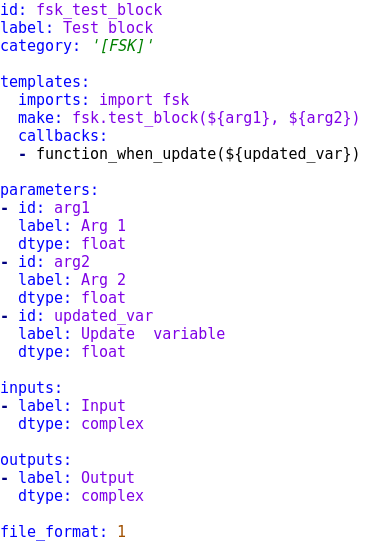
\includegraphics[scale=0.8, left]{figures/Update_yml.png}
    \caption{Example of YAML file of a block which probes the changes made to a variable }
    \label{fig:Update_yml}
\end{figure}


In the Python implementation of the block, the function \texttt{function\_when\_update} needs to be added to the block Python class. It takes as argument the updated value which you can use as you which. In Fig. \ref{fig:Update_python}, an example is provided where we simply change an internal variable of the block.

 \begin{figure}[H]
    \centering
    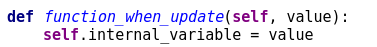
\includegraphics[scale=0.8, left]{figures/Update_python.png}
    \caption{Example of callback function when a variable is updated}
    \label{fig:Update_python}
\end{figure}

Finally, recompile the gr-fsk library, reopen GNU Radio and add the variable that will be updated in the block parameters.

\section{Comments on LimeSDR parameter update}

You can use what you learned in this tutorial to dynamically update some parameters of the LimeSDR, e.g., the threshold of the preamble detector or the RX gain, from a GNU radio block. The structure of the RX chain is shown on Fig. \ref{fig:Structure}.

 \begin{figure}[H]
    \centering
    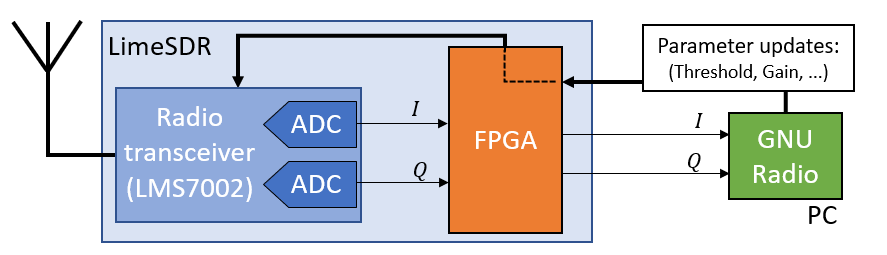
\includegraphics[scale=0.8]{figures/Structure.png}
    \caption{RX chain structure}
    \label{fig:Structure}
\end{figure}

However, we need to highlight an important point. GNU radio works with buffer of data. When you make modifications to some LimeSDR parameters, it will be done almost immediately, but GNU radio has already multiple hundreds or thousands of samples waiting in a buffer, not affected by this modification. For example, if you modify the threshold or the gain, you will still have samples that arrive below your new threshold or with your old gain. We can refer to those unaffected samples as the latency. Fig.\ref{fig:Structure_delay} summarize this idea. As annotated, we can observe a latency up to 25000 samples (62 ms when converted).  You should therefore be careful as updating parameters of the LimeSDR during a packet will probably not affect it. However, it might still be interesting to update parameters from packet to packet.

 \begin{figure}[H]
    \centering
    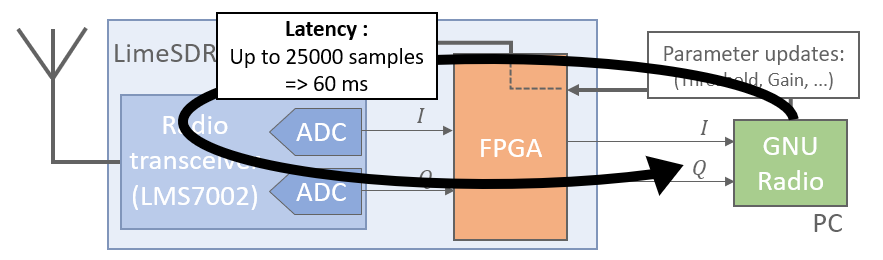
\includegraphics[scale=0.8]{figures/Structure_delay.png}
    \caption{Representation of the RX chain delay when updating LimeSDR parameters from GNU Radio}
    \label{fig:Structure_delay}
\end{figure}
